\documentclass{article}
\PassOptionsToPackage{dvipsnames}{xcolor}
\usepackage{arxiv}

\usepackage[utf8]{inputenc} % allow utf-8 input
\usepackage[T1]{fontenc}    % use 8-bit T1 fonts
\usepackage[hidelinks]{hyperref}       % hyperlinks
\usepackage{url}            % simple URL typesetting
\usepackage{booktabs}       % professional-quality tables
\usepackage{amsmath,amssymb,amsthm}
\usepackage{amsfonts}       % blackboard math symbols
\usepackage{nicefrac}       % compact symbols for 1/2, etc.
\usepackage{makecell}
\usepackage{microtype}      % microtypography
\usepackage{mathrsfs}
\usepackage{float}
\usepackage{graphicx}
\usepackage{doi}
\usepackage{acronym}
\usepackage{listings}
\usepackage{siunitx}
\usepackage{tabularx}
\usepackage{tikz}
\usepackage[dvipsnames]{xcolor}

\usetikzlibrary{trees}

\def\checkmark{\tikz\fill[scale=0.4](0,.35) -- (.25,0) -- (1,.7) -- (.25,.15) -- cycle;}
\def\cross{\tikz\draw[scale=0.3, black, line width=0.3mm](0,0) -- (1,1) -- (0.5,0.5) -- (0,1) -- (1,0) -- (0.5,0.5);}

\newacro{abm}[ABM]{Agent-Based Model}
\newacro{cabm}[CABM]{Cellular Agent-Based Model}
\newacro{ca}[CA]{Cellular Automaton}
\newacro{ib}[IB]{Individual-Based}
\newacroplural{ca}[CA]{Cellular Automata}
\newacro{cpm}[CPM]{Cellular Pottes Model}
\newacro{ecoli}[\textit{E.coli}]{\textit{Escherichia coli}}
\newacro{bsubtilis}[\textit{B.subtilis}]{\textit{Bacillus subtilis}}
\newacro{paeruginosa}[\textit{P.aeruginosa}]{\textit{Pseudomonas aeruginosa}}
\newacro{pg}[PG]{peptidoglycan}
\newacro{a22}[A22]{S-(3,4-Dichlorobenzyl)isothiourea}
\newacro{mre}[\textit{mre}]{murein formation gene cluster E}
\newacro{tirf}[TIRF-M]{total internal reflection fluorescence microscopy}
\newacro{ecm}[ECM]{extracellular matrix}
\newacro{flavo}[\textit{F. johnsoniae}]{\textit{Flavobacterium johnsoniae}}
\newacro{serratia}[\textit{S. marcescens}]{\textit{Serratia marcescens}}

\newcommand{\todo}[1]{\colorbox{WildStrawberry}{\textcolor{white}{#1}}}
\newcommand{\R}{\mathbb{R}}
\newcommand{\denovo}{\textit{de novo}}

\title{Spatial Models of Rod-Shaped Bacteria - From Single-Cell Essays to Collective Phenomena}

%\date{September 9, 1985}	% Here you can change the date presented in the paper title
%\date{} 					% Or removing it

\author{
    \href{https://orcid.org/0009-0001-0613-7978}{
        \includegraphics[scale=0.06]{orcid.pdf}
        \hspace{1mm}Jonas Pleyer
    }
    \thanks{
        \href{https://jonas.pleyer.org}{jonas.pleyer.org},
        \href{https://cellular-raza.com}{cellular-raza.com}
    }\\
	Freiburg Center for Data-Analysis and Modeling\\
	University of Freiburg\\
	% \texttt{jonas.pleyer@fdm.uni-freiburg.de} \\
	\And
    \hspace{1mm}Toquinha-Orelia Bergmann\\
	Freiburg Center for Data-Analysis and Modeling\\
	University of Freiburg\\
	%% examples of more authors
	\And
	\href{https://orcid.org/0000-0002-6371-4495}{
        \includegraphics[scale=0.06]{orcid.pdf}
        \hspace{1mm}Christian Fleck
    }\\
	Freiburg Center for Data-Analysis and Modeling\\
	University of Freiburg
}

% Uncomment to remove the date
%\date{}

% Uncomment to override  the `A preprint' in the header
\renewcommand{\headeright}{Preprint}
%\renewcommand{\undertitle}{Technical Report}
\renewcommand{\shorttitle}{Spatial Models of Rod-shaped Bacteria}

\usepackage{enumitem}
\setlist{nolistsep}

%%% Add PDF metadata to help others organize their library
%%% Once the PDF is generated, you can check the metadata with
%%% $ pdfinfo template.pdf
\hypersetup{
pdftitle={Spatial Models of Rod-shaped Bacteria},
pdfsubject={q-bio.NC, q-bio.QM},
pdfauthor={Jonas Pleyer, Christian Fleck},
pdfkeywords={},
}

% Change numbering of equations
% \numberwithin{equation}{section}

\begin{document}
\maketitle

% TABLE OF CONTENTS
% Remove this before submission

%###################################################################################################
\begin{abstract}
    % \begin{itemize}
    %     \item Rod-shaped bacteria are everywhere
    %     \item many different species
    %     \item Shape plays crucial role in many effects such as motility, growth, collective effects etc.
    %     \item How does the behaviour of individual cells lead to collective phenomena?
    %     \item Mathemtical models help us to understand this
    %     \item We provide review of current state
    %     \item question; which biological required? answer: mesoscopic; want to get to emergent
    %         collective phenomena from single-cell behaviour
    % \end{itemize}
    Rod-shaped bacteria are ubiquitous forms of life which can be found in diverse microenvironments
    encompassing a wide, diverse range of species.
    Their elongated shape plays a crucial role in many biological processes such as enhancing
    swimming capabilities or promoting surface interactions.
    A key question is how the individual behaviour of multiple bacteria can lead to emergent
    spatial phenomena such as swarming and biofilm formation.
    Mathematical and computational methods provide powerful tools which allow researchers to bridge
    this gap and analyze the impact of various single-cell processes systematically.
    In this review we capture the current state of mathematical and computational approaches,
    emphasizing flexible, mesoscopic models which can be adjusted to describe a wide range of
    biological processes at their respectively required level of detail in order to study a variety
    of collective effects.
    We come to the conclusion that mechanical properties have been investigated extensively while
    other biolgical effects such as extracellular signalling, growth and differentiation are less
    studied.
\end{abstract}

% keywords can be removed
\keywords{Spatial \and Modeling \and Rod-Shaped \and Bacteria \and Mathematics}

% \textbf{POSSIBLE TITLES}
% \begin{itemize}
%     \item Mechanical Models of Rod-Shaped Bacteria - From Single-Cell Modeling to Collective Phenomena
%     \item Mathematical Modeling of Rod-Shaped Bacteria - From Single-Cell Mechanics to Collective Phenomena
%     \item Mathematical Models of Rod-Shaped Bacteria - From Single-Cell Analyses to Collective Phenomena
% \end{itemize}

\vfill
\pagebreak
\tableofcontents
\vfill
\pagebreak


%###################################################################################################
\section{Introduction}

\todo{move this to introduction}
Bacteria, unicellular divers procaryotic organisms and one of the simpler model to study individual single cell morphogenic changes up to emergent spatial emergent phenomena \cite{Vollmer2001}.
Various cell shapes are encountered in the prokaryotic world/Contain cells of different shapes, and yet we know little about how these shapes affect community biology \cite{Smith2017}.

Among the Well-studied examples include rod-shaped bacteria. Including gram negative as well as gram positive bacteria \ac{ecoli} (a Gram-negative bacterium) and \ac{bsubtilis} (Gram-positive) \cite{Chang2014}.

Including gram negative as well as gram positive bacteria \ac{ecoli} (a Gram-negative bacterium) and \ac{bsubtilis} (Gram-positive) \cite{Chang2014}.

\begin{itemize}
    \item Interested in all variations of rod-shaped bacteria; stiff, flexible, spiral, etc.
    \item Einordnung in andere Bakterienarten
    \item Rods are "more fundamtenal" than spheres (cocci) (which citation?)
    \item mesoscopic approach; take what cellular behaviour we need; interested in multicellular
        dynamics ultimately
    \item Talk about differences between: Gram-Positive, Gram-Negative
    \item Morphologies: Bacilli, Corkscrew, Filamentous, Spirochete
\end{itemize}

Order of this review
\begin{enumerate}
    \item Describe Biological Reality of Rod-shaped bacteria; single-cell; emergent phenomena
    \item What do we need within a model?
    \item Discuss modeling approaches; Mathematical, Computational
    \item Compare reusable computational tools
    \item Can we estimate their parameters?
\end{enumerate}

\section{Biological Building Blocks}
\subsection{Cell Shape}

\textbf{TODO Put a disclaimer here that says that we do not treat every aspect, but try to focus on
stuff which is important for us.}

\begin{enumerate}
    \item Cell wall and cytoskeleton fundamental as building blocks of cell shape
    \item How are they coupled?
    \item Describe mechanics of growth in rod-shaped bacteria
    \item How do single machineries regulate rod shape maintenance/shape?
    \item How does Division work?
    \item Brief outlook to other forms
\end{enumerate}

\subsubsection{Cell Wall, Cytoskeleton \& Interplay}

The shape of bacteria is mainly determined by their envelope and its growth. Most bacteria are surrounded by peptidoglycan \ac{pg}, a mesh-like macromolecule of glycan strands that are crosslinked via short peptides, which is chemically unique to bacteria~\cite{Cava2014, Amir2014, Cochrane2020}. This essential structure mechanically resists high turgor pressure, giving the cell its specific shape, isolating and regulating environmental uptake, which is indispensable for bacterial survival~\cite{Cochrane2020, vanTeeffelen2018}.

Although rod morphology is physically defined by \ac{pg}, the rod shape requires cytoskeletal support. At the end of the last century, an actin-like protein MreB was discovered~\cite{Erickson2001}.  It's crystal structure \cite{Lowe2017_lj} and filament-forming dynamic \cite{Dersch2020} show strong similarity to actin. Additional actin-homologues, MreC, and MreD were later identified \cite{vandenEnt2001}.

MreB filaments make/form a spiral-like or banded pattern along the length of the cell, moving circumferentially around the rod, coordinating \ac{pg} synthesis \cite{Garner2021, White2012, López2006}. Thus, MreB polymers' dynamics actively restrict and/or control the mobility of cell wall elongation complexes \cite{DEscobar2011}, thereby linking cytoskeletal organisation with local changes of cell shape \cite{Shi2018}. MreB filaments are attracted to regions of negative Gaussian curvature and excluded from regions of positive Gaussian curvature, such as the cell poles, contributing to a rod-shaped \cite{vanTeeffelen2018}. The transmembrane protein, like RodZ, modulates MreB curvature preference \cite{Bratton2018}, altering MerB localisation and density. 


\paragraph{Cell Wall}
\begin{itemize}
    \item \cite{Cava2014} main cell envelope of bacteria is a mesh-like macromolecule of glycan strands that are crosslinked via short peptides. Thus  peptidoglycan \ac{pg}
    \item \cite{vanTeeffelen2018} \ac{pg} PG meshwork mechanically resists the high turgor pressure and gives the cell its specific cell shape
    \item \cite{Cochrane2020} \ac{pg} chemically unique (to bacteria) and essential for cell survival. Therfore it's synthesis and turnover is targeted by a range of antibacterial treatments
        Different mechanism based on use of polar growth zones derived from the division machinery (\ac{pg} and FtsZ)
    \item \cite{Amir2014} bacterial cell shape is physically determined by the \ac{pg} cell wall but not sufficient for maintaining rod-shape on its own, need more effects \todo{do we need more details from this paper?}
\end{itemize}

\paragraph{Cytoskeleton}
\begin{itemize}
    \item It was long believed that bacteria lack cytoskeletal filaments but with the end of the last century, it was discovered that the MreB protein fills this role since it "[..] forms an actin-like cytoskeleton in bacteria [..]" \cite{Erickson2001}.
    \item \cite{Dersch2020} It can polymerize and form filaments which behave similar to actin microfilaments 
    \item \cite{Lowe2017_lj} Studies of its crystal structure further showed the similarity to actin~\cite{vandenEnt2001} and the MreB, MreC and MreD proteins were identified as homologues of actin 
    \item \cite{Bratton2018} trans-membrane protein RodZ can modulate MreB density. It has a direct effect on MreB curvature preference
\end{itemize}

\paragraph{Interplay}
\begin{itemize}
    \item \cite{White2012} \cite{López2006} MreB adopts a spiral-like or banded pattern along the length of the cell coordinating \ac{pg} synthesis  
    \item  \cite{Shi2018} MreB filaments move circumferentially around rods \cite{Garner2021} of any width, resultant \ac{pg} synthesis around the rod circumference is stabilizing rod shape against the internal pressure
    \item \cite{Shi2018} MreB is a cytoskeletal organizing element it's localization also directs cell growth to locally change cell shape 
    \item \cite{vanTeeffelen2018} MreB filaments are attracted to regions of negative Gaussian curvature and excluded from regions of positive Gaussian curvature, such as the cell poles, contribtuting to a rod-shape
    \item \cite{DEscobar2011} MreB polymers actively restrict and/or control the mobility of cell wall elongation complexes
    \item \todo{not used following two}
    \item \cite{Wang2010, Wang2010_protocol} MreB and \ac{pg} contributes to nearly equal parts to the stiffness of a cell
    \item \cite{Olshausen2013} got good resolution of MreB dynamics with the help of \ac{tirf}. Their mathematical model confirms that MreB acts as mechanical organizer, coupling the cytoskeleton with cell wall synthesis to maintain rod shape.
\end{itemize}

\subsubsection{Growth, Maintenance \& Division}
\paragraph{Growth}
\begin{itemize}
    \item \cite{Daniel2003} 2 ways maintaining rod shape: with/without MReB: A few rod-shaped bacteria have no MreB system. MreB-guided lateral wall growth or polar elongation
    \item \cite{Cooper1991} \cite{Wang2010_2} \ac{pg} synthesis is spatially and temporally regulated. During elongation, cells grow at a constant diameter, expanding surface mainly along the sidewall. During constriction polar synthesis is initiated forming new polar caps
    \item \cite{Chatterjee1988} spatial variation of mechanical stress in the cell also contributes to growth patterns, shape maintenance, and division site selection.
    \item \cite{Chang2014} cell elongation is comparable for gram-negative and gram-positive bacteria (\ac{bsubtilis} and \ac{ecoli}) despite their wall thickness
    \item \cite{Billaudeau2017} wall thickness influence elongation dynamics (species-specific coordination) (details if needed: in \ac{bsubtilis} and \ac{ecoli} \ac{pg} assembly, spatial pattern, wall thickness, and machinery organization differ, leading to distinct elongation dynamics )
    \item \cite{DePedro2003} new \ac{pg} is inserted in discrete patches along the lateral sidewall
    \item \cite{Billaudeau2017} Growth is MreB-dependent, maintaining constant diameter
    \item \cite{Si2015} Bacterial morphogenesis and \ac{pg} synthesis are mechanically sensitive, showing that growth patterns are adaptive and coupled to physical forces.
\end{itemize}

\paragraph{Maintaining/Loosing Rod-shape}
\begin{itemize}
    \item \cite{Jones2001} MreB is responsible for cell width regulation and Mbl is responsible for linear axis regulation. Beyond rod-shaped bacteria.
    \item \cite{Lleo1990} shape is balanced by two reaction i) wall elongation ii) septum formation. cocci shaped lost i) or are induced by mutations in i)
    \item e.g. for lacking i): \ac{a22} treated cells \cite{IWAI2002}, \textit{rodZ} deletion mutants \cite{Shiomi2008} and \ac{mre} mutants \cite{Wachi1987} were found to induce spherical cells shape indicating that cell shape maintenance involves proteins encoded by the \ac{mre} like MreB or interacting with them
    \item extension to point before: specifying what \ac{a22} is. \cite{Bean2009} \ac{a22} binds directly to nucleotide-free MreB, due to its high affinity to the nucleotide-binding pocket of MreB. Thereby disrupting MreB assembly
    \item Switch in or \denovo \ac{pg} synthesis is sufficient to regenerate the cell wall and restore a rod-shape morphology \cite{Huan2021} spherical to rod-shape  \cite{Kawai2014} L-form to rod-shape
    \item \cite{Garner2021} MreB filaments move circumferentially around rods of any width, but filament motion was isotropic in spherical cells, moving in all directions\todo{why are we citing this?}
\end{itemize}

\paragraph{Cell division}
\begin{itemize}
    \item \cite{Bramkamp2009} Two inhibitory systems regulates the assembly FtsZ \cite{Oliva2004}: i) Min system prevents division near poles and ii) nucleoid occlusion prevents cell division over the nucleoids
    \item adding to first point \cite{Koch1995} \cite{Chatterjee1988} central FtsZ-ring assembly is favored by mechanical forces. Its regulation is thereby a combination of mechanical cues and biochemical regulation
    \item FtsZ filaments are forming a ring (Z-ring) at division site \cite{Li2007} generating constriction force for division. The ring tension is regulating \ac{pg} synthesis \cite{Lan2007}
    \item \cite{DenBlaauwen2008} divisome or septosome switches \ac{pg} synthesis from dispersed to a concentrated local to from new cell poles
    \item \cite{Woldringh1987} \cite{Cooper1991} surface synthesis rate increase at the start of constriction, elongation and pole formation use distinct, spatially regulated \ac{pg} insertion modes, supporting the idea of separate elongation and division machineries (divisome/septosome)
    \item \cite{Kruse2005} \cite{Gitai2005} MreB contributes in forming a bacterial mitotic-like machine and control Bacterial DNA segregation
    \item \cite{Karczmarek2007} DNA and origin region segregation are not affected by the transition from rod to sphere after inhibition of Escherichia coli MreB by \ac{a22} \todo{do we really need this extra information?}
    \item \cite{denBlaauwen2018} bacterial morphogenetic is plastic and can be reprogrammed changing growth and division axis \todo{@toqi do we really need this for modelling EMERGENT phenomena?}
    \item \cite{Stewart2005} despite symmetric division aging and mortality can occur by asymmetric inheritance of cellular damage (older “mother” cell poles accumulate damage or growth defects over generations)
\end{itemize}

\subsubsection{Rod vs other shape (To Rod or not to Rod?)}
\paragraph{Rod-shape vs. other shape}
\begin{itemize}
    \item \cite{Young2006} shape is an evolutionary trait which influence nutrient uptake, cell division and segregation, adhesion, passive and aktive motility, predator avoidance, and cellular differentiation.
    \item e.g. for point before: \cite{Takeuchi2005} changed \ac{ecoli} morphologies without altering any additional biochemical or genetic functions and automatically altered cell motility
    \item Other shapes often request other or additional cell-wall-machineries \cite{Zapun2008} or cytoskeletal components like crescentin which are bacterial equivalent to intermediate filaments (IFs\cite{Ausmees2003}
    \item to conclude: \cite{Jones2001} "We therefore suggest that a sphere is the default shape taken by cells in the absence of an active, mreB-dependent shape determining system, and that more complex shapes are usually determined in part by \textit{mreB} systems". \cite{Young2006} "It can be argued that the earliest cells consisted of "[...] rods and filaments with cocci being
\end{itemize}

\subsection{Reaction to Environmental Factors}
\subsubsection{Taxi}
\begin{itemize}
    \item \cite{Krell2011} multiple diverse taxis systems integrating chemical (chemotaxis), light (phototaxis), oxygen (aerotaxis), temperature (thermotaxis), and magnetic fields (magnetotaxis) stimuli. Bacterial taxis are versitle and highly evolutionary adapted to the species environment.
    \item \cite{Nikita2009, Bourret2002} Chemotaxis, is the most common and best studied form of taxis. It is a receptor-mediated signaling network that integrates external chemical cues to modulate flagellar motion and control movement direction.
\end{itemize}

\subsubsection{Nutrient uptake/distribution}
\begin{itemize}
    \item \cite{Davies2021, Niederweis2008, Tanaka2018} Bacterial nutrient uptake is mediated by highly selective transporter systems (e.g., ABC transporters, TRAP systems, and PTS) that import sugars, amino acids, ions, carbon, nitrogen, iron, and lipids; bacteria can also modulate cell envelope permeability and secrete enzymes to facilitate nutrient acquisition
    \item \cite{Velicer2009,Rory2015} a diverse part of bacterial are predators and found in various environments, plaing a significant role in microbial community structure and dynamics, with different modes of predation and independent evolutionary origins
    \item \cite{Caron1994} Bacteria acquire significant nitrogen and phosphorus from dissolved inorganic nutrients, competing with phytoplankton and influencing the microbial loop; overall contribution to ocean nutrient uptake is poorly understood
    \item \cite{Watteaux2015} Motile chemotactic bacteria have an enhances nutrient uptake rate. 2.2 times faster than non-motile 
    \item \cite{Li2025} matrix-producing improve access to nutrients, supporting growth under nutrient-limited conditions
\end{itemize}

\subsubsection{Movement (swimming, gliding, recipe for swarming)}
\begin{itemize}
    \item \textbf{swimming}
    \item \cite{Shen2022} bending stiffness of the flagellar filament support propulsion and reorientation during swimming, it does not vary
    \item \cite{Kong2014} swimming motion of rod-shaped magnetotactic bacteria is regulated by shape and magnetism
    \item \cite{Alberti1990} swimming cells are short, mononucleate, flagellated for planktonic motility. Can differentiate to swamers, when growing on and surface
    \item \textbf{swarming}
    \item \cite{Harshey2015} compared to swimming which direct a single through chemotaxis to find nutrients and avoid toxic environments swarming is a collective motion suppressing chemotaxis and using the dynamics of their collective motion to continuously expand and acquire new territory
    \item \textbf{gliding}
    \item \cite{ContrerasM2024} gliding relies on a outer-membrane complex that attaches the substrate at fixed sites of focal adhesion enabling directional gliding motility
    \item \cite{Chang2016}type IV pili generates retraction force for twitching motility, pulling the cell across surfaces 
    \item \cite{Shah2022} model shows that non-Newtonian slime behavior enhances gliding motility by optimizing force transmission and energy use
    \item \cite{Shrivastava2015} \ac{flavo} and \textit{Myxococcus xanthus} are gliding rod-shpaed flagelaten-free spicies. Their gliding relies on rotary motors driving mobile surface filaments, providing continuous propulsion analogous to a snowmobile
\end{itemize}

\subsubsection{Cell-Cell Forces/Adhesion/Friction}
\begin{itemize}
    \item \textbf{adhesion}
    \item \cite{vanLoosdrecht1989, Hori2010} Bacterial adhesion is driven by physicochemical interactions: van der Waals, electrostatic, hydrophobic, and acid-base forces and it's strength is determined by both surfaces properties (charge, hydrophobicity, roughness) determine
    \item \cite{BrettFinlay2014, Berne2018} Adhesins, pili/fimbriae, and surface proteins mediate the binding to \ac{ecm} components/ adhesion is a highly heterogeneous and dynamic process. Binding to a host \cite{Beachey1981, Vaca2019}
    \item \cite{Vaca2019,Beachey1981} Gram-negative bacteria (eg. \ac{ecoli}) express outer membrane proteins (adhesins) which allow them to attach to various hosts
    \item Type IV pili \cite{Ellison2021} or flagella in general \cite{Haiko2013} are more than force-generating structures that coordinate bacterial movement, they play an important role in the direct adhesion, and environmental interaction
    \item \textbf{cell-cell forces}
    \item some bacteria can fuse to each other when they are long enough at close distance \cite{Kudryashev2011}
    \item \todo{More about friction/physical cell-cell interactions}

\end{itemize}

\subsubsection{Adaptation}
\begin{itemize}
    \item \cite{Bertrand2019} bacteria encountering new nutrients have an adaptive phase: lag-phase in which there is now division. While this dormant stage metabolic adaptation and macromolecular synthesis occur to prepare  for rapid cell growth and robust cell division
    \item \cite{Senkei2007} Bacterial populations exhibit heterogeneous, asynchronous responses in lag times, swimming speeds, or surface motility activation for adaptive advantage
    \item \cite{Barrangou2007} CRISPR provides adaptive resistance against bacteriophages \cite{Duckworth2002} in prokaryotes (\cite{Borges2017} some protein families have anti-CRISPR function)
    \item \cite{Amir2014_2} elastic deformations after pulse-like force do not change the shape permanently. Plastic deformations occur adapting to external bending forces causing the cell walls to grow differentially leading to persisting plastic deformations
    \item \cite{Kim2003, Lai2009} Swarm-cell have elevated resistance to multiple antibiotics
    \item \cite{Huan2021, Errington2020, Licking2000, Barák2019} a variety of bacteria can form spores in order to survive under unfavorable environmental conditions. Germination, these spores restore vegetative morphology
    \item \cite{Licking2000, Jose2016, Branda2001} certain bacteria from fruiting bodies, a multicellular aggregation of differentiated cells, where spore formation is preferred
\end{itemize}

\subsection{Living as a Community}

\subsubsection{Quorum Sensing}
\begin{itemize}
    \item \cite{Stephen2007} Bacteria produce and secrete small signaling molecules called autoinducers called Quorum sensing. Coordinate gene expression collectively, enabling adaptive group behavior
    \item \cite{MorenoGmez2023} Quorum sensing allows bacteria to collectively process information enhancing decision accuracy through population-level coordination
    \item \cite{Hense2007, Boyer2009}  Quorum sensing not only within single species, but also interspecies and cross-kingdom (e.g., bacteria-host, bacteria-virus). \cite{Liu2025} Highlights some applications in biomedical and environmental technologies 
    \item \cite{Solano2014} Quorum sensing plays a key role in mature biofilms for e.g transition from a sessile community to a free-living state
\end{itemize}

\subsubsection{Differentiation}
\begin{itemize}
    \item \textbf{swarming}
    \item \cite{Harshey1994} swarming is active and rapid surface motility. Swarmer cell is are usually long, multinucleate, hyperflagellated bacterial cell
    \item \textbf{sporilation}
    \item some bacterial can have lifecycle like Myxococcus xanthus \cite{Jose2016}  \ac{bsubtilis} \cite{Branda2001} for e.g task division and environmental adaptation
    \item \cite{Licking2000}  Myxococcus xanthus have starvation-dependent and starvation-independent pathways of sporulation and produce structurally different spores
    \item \cite{Barák2019} \ac{bsubtilis} can divide asymmetrically during sporulation one cell differentiation process 
    \item \textbf{fruiting bodies}
    \item \cite{Huan2021} Myxococcus xanthus sporulat and make fruiting bodies. 
    \item \textbf{task division}
    \item \cite{Lopez2010} Extracellular signalling in \ac{bsubtilis} orchestrates diverse, co-existing cell fates via specific signal-sensor-regulator cascades, enabling a community of genetically identical cells to specialize into distinct roles.
    \item \cite{Flemming2016} cellular differentiation/task division in biofilms (matrix production, motility, sporulation)

\end{itemize}

\subsubsection{Biofilms}
\begin{itemize}
    \item \cite{Dunne2002} Bacterial adhesion is a dynamic, regulated process that underlies biofilm formation and persistence on diverse surfaces
    \item \cite{Flemming2016} “Biofilms: an emergent form of bacterial life” names emergent phenomena: Enhanced stress tolerance, Collective resource capture, Spatial organization and division of labor, Self-structuring and architecture formation
    \item \cite{Wisnu2022} Mixed-species biofilms have enhanced survival, mediated by antimicrobial-resistant keystone species
    \item \cite{Ong1999, vanLoosdrecht1989, Hori2010} initial colonization and biofilm potential is governed by the bacterial features and biomaterial properties
    \item \cite{Rendueles2012} Competition in biofilms has a key role. Rivality in surface-colonisation leads to strategies that target adhesion, signalling and matrix dynamics allowing mixed-species biofilms to regulate neighbour entry and community structure
    \item following points are already in text
    \item \cite{Duvernoy2018} shaping early biofilm morphogenesis by asymmetric adhesion of rod-shaped bacteria to surfaces early biofilm transition architecture from 2D to 3D structure when confinement and under mechanical forces.
    \item \cite{Grant2014} Elasticity of the bacterial cells and elastic interactions plus the frictional forces between the bacteria and the surrounding agarose medium are key features of the 2D to 3D transition
\end{itemize}

\section{Mathematical \& Computational Frameworks}

\paragraph{Spatial Colony Organization}
\begin{itemize}
    \item \cite{Ingham2008} Swarming behavior with collective motility and chemotactic interactions dominates colony organization, leading to dynamic branching and vortex-like patterns
    \item \cite{Starru2007} while non-chemical, physical cell-cell interactions drive emergent collective motion patterns such as vortices and streams. Cell shape as the length-to-width ratio controls the level of clustering thereby strongly influencing swarm dynamics.
    \item \cite{Jin2020} adhesion, friction, and cell stiffness influence colony morphology- stronger cell-cell adhesion leads to denser, slower-growing biofilms, while weaker adhesion promotes faster spreading
    \item \cite{Trejo2013} \ac{bsubtilis} pellicles is mechanically driven process, where extracellular matrix elastity leads to wrinkled morphology
    \item \cite{Li2025, vanGestel2015} biofilm expansion relies on division of labor. Surface-colonising regulated by cell differentiation. i) matrix-producers forming aligned bundels(“van Gogh bundles”) which physical properties set the expansion rate of the colony ii) surfactin-producers reduce surface friction.
    \item \cite{Dong2022} mechanical organization contributes to community robustness. biofilm self-healing mechanisme by reconnecting and regrowing van Gogh bundles 
    \item \cite{Buka1987} "For example, injection of a flux of a liquid crystal between two close parallel plates (viscous fingering) causes orientation of the molecules to couple with the flow, with the resulting emergence of dendritic patterns." (Wikipedia)
\end{itemize}

\paragraph{Toqi suggest those for modeling section}
\begin{itemize}
    \item \cite{Moreau2018} theoretical study abut asymptotic coarse-graining model for slender rods, biofilaments, and flagella
    \item \cite{Nagarajan2022} Agent-Based Modeling of Microbial Communities \todo{use contents of this review}
    \item the DLVO-theory~ \cite{Verwey1947,Derjaguin1993} \todo{do we need those later?}
\end{itemize}

\subsection{Modeling Aspects}

\begin{itemize}
    \item aspect groups (C), (CC), (CE) are related to computational approaches\\
        for c in cells\\
        for c1 in cells: for c2 in cells: calculate\_interaction(c1, c2);\\
        for c in cells; interact\_with\_domain(c, domain);
\end{itemize}

\begin{figure}
    \centering
    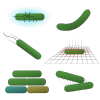
\includegraphics[width=0.5\textwidth]{figures/concept-figure.png}
    \caption{TODO}
    \label{fig:concept-figure-aspects}
\end{figure}

\begin{itemize}
    \item biological phenomena have been summarized before
    \item emphasize: more than just mechanics, also incorporate cell-cycle, extracellular
        reactions, (polar) interactions, etc.
    \item present "grouping" of biological phenomena into: (C) Cellular, (CC) Cell-Cell, (DC)
        Domain-Cell aspects \textbf{TODO possibly rename Domain to Environment}
    \item explain aspect-groups
    \item discuss table \ref{table:simulation-aspects}
\end{itemize}

\begin{table}[H]
    \newcounter{aspect}
    \setcounter{aspect}{1}
    \newcommand{\asp}{(\arabic{aspect}\refstepcounter{aspect})}
    \centering
    \def\arraystretch{1.3}
    \begin{tabularx}{\textwidth}{c l X}
        &\textbf{Aspect} & \textbf{Description}\\
        \toprule
        &\textbf{(C) Cellular}\\
        \midrule
        \asp & Rod-Shaped Mechanics &
            Rod-shaped bacteria are flexible rods which are able to freely move around (off-lattice
            approach) \cite{Takeuchi2005,Ursell2014,Amir2014_2}.\\
        \asp & Movement &
            \textbf{TODO} Flagellum, Swimming\\
        \asp & Growth &
            Cells grow exponentially by inserting new material either along the circular part of the
            rod or at the tip~\cite{Robert2014,Takeuchi2005}.\\
        \asp & Differentiation &
            \textit{B.subtilis} is known to differentiate into matrix-producing and
            surfactin-producing cells \cite{vanGestel2015,Lopez2010}.\\
        \asp & Division &
            The formation and continuation of van Gogh bundles is driven by cell division
            \cite{vanGestel2015}.
            Bacteria can form multilayers during their growth phase \cite{Duvernoy2018}.\\
        \asp & Variable Parameters &
            Parameters for individual cells are not fixed values but rather taken from a
            distribution \cite{Koutsoumanis2013}.\\
        &\textbf{(CC) Cell-Cell Interactions}\\
        \midrule
        \asp & Adhesion &
            Bacteria adhere to each other at longer distances and attach when in close contact
            \cite{Verwey1947,Trejo2013}.
            The interaction between rods can be polarized \cite{Duvernoy2018}.\\
        \asp & Friction &
            Friction between cells \cite{Grant2014} can be asymmetrical \cite{Doumic2020}.\\
        &\textbf{(DC) Domain-Cell Interactions}\\
        \midrule
        \asp & External Forces &
            Bacteria tend to stick to surfaces \cite{vanLoosdrecht1989}.
            The extracellular gel exerts a force onto the cells \cite{Grant2014}.\\
        \asp & Extracellular Reactions &
            Bacteria can take up nutrients or possible secrete/take up signalling molecules
            \cite{Li2025}.\textbf{TODO citation signalling}\\
        \bottomrule
    \end{tabularx}
    \label{table:simulation-aspects}
    \caption{TODO}
\end{table}

In order to describe the multicellular systems we looked at in the preceding sections, multiple
different aspects of cellular behaviour and their interactions with the surrounding domain need to
be considered and implemented.
Table \ref{table:simulation-aspects} summarizes these aspects and points to the relevant
experiments.
Aspects (1-5) take place inside the cell, (6,7) correspond to interactions between different
cellular agents and (8,9) to interactions with the domain.
It should be noted explicitly that these simulation aspects can be coupled to each other.
We have already seen such an example in the results of @Takeuchi2005 and @Ursell2014 where the
continued growth modulates the mechanical response of the cell.
Additionally, Aspect (5) is an overarching concept which is relevant for all processes.
Especially for the parameters which facilitate growth, we can assume that there is no direct
inheritance from one generation to the next but only a stochastic distribution of parameters from
which the new value is drawn (see supplement).

\subsection{Computational Modeling Frameworks}

\subsubsection{List Frameworks}
\begin{itemize}
    \item \cite{breitwieser_biodynamo_2022} BioDynamo TODO mention this; I think no support
    \item \cite{Gorochowski2012,Matyjaszkiewicz2017} BSim; has rods
    \item \cite{Kreft1998,Kreft2001} (BacSim) "Individual-based modelling of biofilms Free"
    \item \cite{Kang2014} (Biocellion) only cylindrically-shaped potentials
    \item \cite{Gutirrez2017} \texttt{gro}
    \item \cite{Pleyer2025} \texttt{cellular\_raza}
    \item \cite{Bogdanowski2022} iDynomics \textbf{TODO check how this can model rods (it should)}
    \item \cite{GoiMoreno2015} DiSCUS \textbf{TODO}
    \item \cite{Li2019} NUFEB \textbf{TODO}
    \item \cite{Breitwieser2021} BioDynaMo \textbf{TODO}
    \item \cite{Dang2020} MultiCellSim \textbf{TODO}
    \item \cite{Hoehme2010} Tisim/CellSys \textbf{TODO}
    \item \cite{Grimm2006,Grimm2010} \textbf{TODO} "A standard protocol for describing individual-based and
        agent-based models" and update: \cite{Jang2012}
    \item \cite{Rudge2012} CellModeller, has rod-shaped support and some predefined chemical
        reactions etc.
\end{itemize}

\begin{table}
    \centering
    \begin{tabular}{llll}
        \toprule
        Name                                                & Spherical     & Cylindrical   & Flexible\\
        \midrule
        BioDynamo~\cite{breitwieser_biodynamo_2022}         & Y             & Y             &N\\
        BSim~\cite{Gorochowski2012,Matyjaszkiewicz2017}     & ?             & ?\\
        \bottomrule
    \end{tabular}
    \caption{TODO}
\end{table}

Since the beginning of this decade, multiple tools have emerged which are able to describe living
systems on a cellular individual-based approach in various details.
A good reason for choosing a framework over a purpose-built solution is to follow the Findability,
Accessibility, Interoperability and Reuse) FAIR principles by \cite{Wilkinson2016}.
These criteria have been designed to improve the overall infrastructure surrounding (re)usability of
scholarly data and methods.
In our previous work, we investigated their differences and features and capacity to model
individual behaviour of cells \cite{Pleyer2023}.
Using one of these existing toolkits means that already existing functionality can be used to
develop own models and the produced research results can be fed back to the library for fellow
researchers to reuse.
This begs the question, which of these existing models is able to support the long list of aspects
that we set out to describe with the experimentally gathered evidence.

\subsubsection{Many general-purpose Frameworks lack explicit support for Rod-Shaped Bacteria}
\begin{itemize}
    \item \cite{Ghaffarizadeh2018} PhysiCell; no rods
    \item \cite{Swat2012} CompuCell; uses \ac{cpm}; no rods
    \item \cite{Cooper2020} Chaste; cell-centre and vertex-based; no rods
    \item \cite{Starru2014} Morpheus, uses \ac{cpm}; no rods
    \item \cite{Wei2013} BNSim; cells are spheres
\end{itemize}

Of the most popular frameworks, most do not support rod-shaped bacteria out of the box.
The very popular Cellular Potts Model (CPM) \cite{Graner1992} is mostly applied in 2D and only
represents cells as lattice grid points.
Since CompuCell3D \cite{Swat2012} exclusively builds upon the CPM, it can not model rod-shaped
bacteria.
PhysiCell \cite{Ghaffarizadeh2018} was designed to answer questions surrounding cancer research and
currently only supports spherical agents.
Chaste \cite{Cooper2020} was also designed for cancer research but further targets the heart and
tissues.
Naturally its Agent-Based Model supports cell-centre and vertex-based models but no rod shapes.
Morpheus \cite{Starru2014} also employs the CPM along with other spatial representations such as
vertex-based models or PDEs but has no support for Rod-Shaped bacteria.
Even purpose-built solutions such as BNSim \cite{Wei2013} which specifically targets bacterial
networks, assumes a simplified spherical representation for their bacterial agents.

\subsubsection{Varying Support for Rod-Shaped Bacteria}
\begin{figure}[H]
    \centering
    \includegraphics[width=0.3\textwidth]{example-image-a}
    \includegraphics[width=0.3\textwidth]{example-image-b}
    \includegraphics[width=0.3\textwidth]{example-image-c}
    \caption{TODO: Snapshots of Modeling Frameworks}
\end{figure}

As we have seen, many frameworks do not provide existing functionality for rod-shaped bacteria.
However, some others do have various levels of support.
Biocellion \cite{Kang2014} can model agents with cylindrical interaction potentials but does not
model any of the MreB-related bending and rigidity or polar interactions.
They acknowledge this shortcoming: "Mapping a cell to multiple agents is also necessary to
separately model subcellular compartments [..].
However, Biocellion does not yet support this." \cite{Kang2014}
BSim2.0 represents cells as rigid capsular cells made from a cylindrical center part and two
half-spheres, which are placed at the ends of the cylinder to round out the shape.
In order to calculate interactions between cells, possible overlaps are determined and minimized,
thus determining the position values of the next iteration step.
It also accounts for many other phenomena, which are displayed in \textbf{TODO replace}.
BSim does not consider bending forces for individual cells or polar interactions.
The \texttt{gro} programming language was designed to simulate the growth of colonies and cell-cell
communication.
Its "physics computation has been optimized for rigid rod-shaped bodies, like E. coli bacteria"
\cite{Gutirrez2017}.
They recognize two types of forces which are acting on the cellular agents:
\textit{Local forces} which are calculated between adjacent bacteria and a \textit{global force}
which pushes bacteria outwards of the colony.
The latter of these is a phenomenological implementation of the observed colony expansion and the
associated central pressure with it.
This assumption may yield incorrect results for sparsely populated cases.
The engine is limited to 2D and does not consider polar interactions or bending of the rods.

\subsection{Purpose-Built Models}

\textbf{soft-matter keywords}
filamentous, nematic order

\subsubsection{Soft-matter Studies}
\begin{itemize}
    \item \cite{Duman2018} "Collective dynamics of self-propelled semiflexible filaments"
        (no division, no intracellular dynamics, no growth)
    \item \cite{Joshi2019} "The interplay between activity and filament flexibility determines the
        emergent properties of active nematics"
    \item \cite{Modica2024} "Soft confinement of self-propelled rods: simulation and theory"
    \item \cite{Peruani2006} "Nonequilibrium clustering of self-propelled rods"
    \item \cite{Saintillan2013} "Active suspensions and their nonlinear models" (suspensions of
        self-propelled microorganisms, dynamics of chemotactically responsive)
    \item \cite{Wensink2012} "Meso-scale turbulence in living fluids" (contains coarse-graining)
    \item \textbf{TODO look for more mixed-morphology (rods \& spheres) papers}
\end{itemize}

\subsubsection{Others}
\begin{itemize}
    \item \cite{Rosenberger1978} "Surface growth in rod-shaped bacteria" (Mathematical Model)
    \item \cite{Hsu2009} "A 3D Motile Rod-Shaped Monotrichous Bacterial Model" (Mathematical \&
        Numerical model for rigid rods which move with flagella)
    \item \cite{Hu2015} "swimming properties of an E. coli-type model bacterium are investigated by
        mesoscale hydrodynamic simulations"
    \item \cite{Cooper2006} "we conjecture that the current observed shape of these bacteria may
        have been determined, in part, to obtain the most efficient shape for moving through liquids."
    \item \cite{Schuech2019} \textbf{TODO study this in more detail} take into account curvature;
        have in-silico model
    \item \cite{Cylke2023} growth of \ac{ecoli} might be super-exponential; quantitative analysis of
        "morphogenetic noise"
\end{itemize}

\begin{table}
    \centering
    \begin{tabular}{llll}
        \toprule
        Study       & Rod Type      & Growth        & etc.\\
        \midrule
        \cite{Duman2018} ...\\
        \bottomrule
    \end{tabular}
    \caption{TODO}
\end{table}

\subsubsection{Promosing Candidates}
\begin{itemize}
    \item \cite{Abar2017} "Agent Based Modelling and Simulation tools: A review of the state-of-art software"
    \item other generic frameworks exist, which may allow to model the desired functions
    \item \cite{Winkle2017} "Modeling mechanical interactions in growing populations of rod-shaped bacteria"
    \item \cite{Winkle2021} "Emergent spatiotemporal population dynamics with cell-length control of synthetic microbial consortia"
    \item \cite{Doumic2020} "A purely mechanical model with asymmetric features for early morphogenesis of
  rod-shaped bacteria micro-colony"
    \begin{itemize}
        \item This is a really good paper for referencing
        \item no bending in mathematical model
        \item Compare distributions of "Read-Outs" to data
        \item uses steric force (see also previously \cite{Trejo2013})
    \end{itemize}
    \item \cite{Grant2014} purposely-built model written in `C++`
    \begin{itemize}
        \item describes bacteria as collection of overlapping spheres
        \item spheres are coupled by non-linear springs (Euler-Bernoulli dynamic beam theory);
        This assumption is unfounded; they show however that it does not alter their results in this
        case
        \item only model repulsive forces; no attraction, adhesion
    \end{itemize}
    \item \cite{Cho2007} only 2D, no bending, no parameter estimation; based on work done in 
        \cite{Jnsson2005}
    \item \cite{Storck2014} TODO;
    41 Parameters for various cases;
    only 8 parameters taken from literature values/quantified;
    generated growth rate randomly (normal distribution), but for each growth step; this is
      stochastically equivalent but numerically slightly more intense;
    \item \cite{Volfson2008} TODO; continuum model, equations of nematodynamics \cite{Doi1988-ad}
    \begin{align}
        \partial_t \rho + \partial_z (\rho \nu) &= \alpha \rho\\
        \partial_t q + \nu \partial_z q &= B(1-q^2) \partial_z \nu\\
        \partial_t(\rho \nu) + \nu \partial_z (\rho \nu) &= - \partial_z p - \mu \rho \nu
    \end{align}
    \item \cite{Pleyer2023} TODO "Modeling mechanical interactions in growing populations of
        rod-shaped bacteria"
    \item \cite{Kong2014} TODO "Swimming motion of rod-shaped magnetotactic bacteria: the effects of
        shape and growing magnetic moment"
    \item \cite{Constantino2016} "Helical and rod-shaped bacteria swim in helical trajectories with
        little additional propulsion from helical shape"
    \item \cite{Starru2007} TODO very interesting FEM-based model
    \item \cite{Martins2015} "'miSimBa' — A simulator of synthetic time-lapsed microscopy images of
        bacterial cells"
    \item \cite{You2018} Hard-Rod model, continuous model
    \item \cite{Valdez2025} "Biomechanical modeling of spatiotemporal bacteria-phage competition"
    \item \cite{Schwarzendahl2022} "Do active nematic self-mixing dynamics help growing bacterial colonies to maintain local genetic diversity?"
\end{itemize}

\subsection{Parameter Estimation \& Techniques}

\subsubsection{Papers which did some sort of parameter estimation}
\begin{itemize}
    \item \cite{Storck2014} TODO; 41 Parameters for various cases; only 8 parameters taken from
        literature values/quantified
    \item Highlight lack of estimation of mechanical parameters for Agent-Based Models
    \item \cite{Gallaher2017} TODO "Hybrid approach for parameter estimation in agent-based models"
    \item \cite{Nguyen2024} TODO tracking single cells; but then do bulk analysis with them, no
        rod-shaped bacteria
    \item \textbf{TODO add more of the soft-matter papers}
    \item \textbf{TODO see if any of the frameworks do have estimates}
\end{itemize}

\begin{figure}
    \centering
    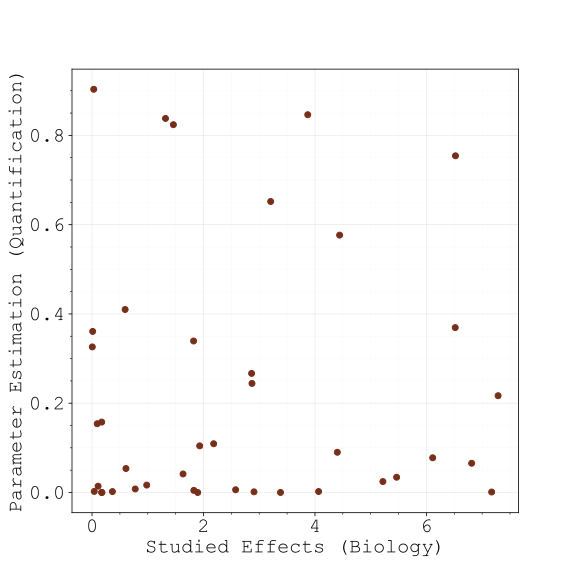
\includegraphics[width=0.5\textwidth]{figures/studies-scatterplots.pdf}%
    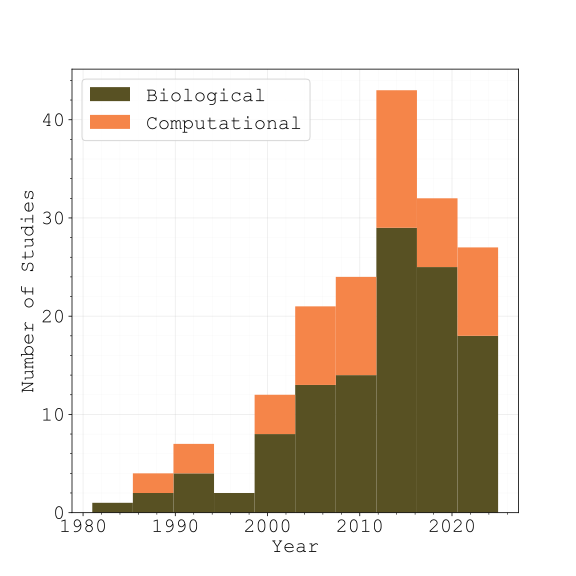
\includegraphics[width=0.5\textwidth]{figures/studies-over-time.pdf}
    \caption{
        TODO FAKE FIGURES. Peak at $\approx2008$ likely comes from CRISPR Cas.
    }
\end{figure}

\subsubsection{Strategies for comparing simulation with data}
\begin{itemize}
    \item Simply do not compare: "Biolgically-inspired"
    \item Select specific feature to investigate
    \begin{itemize}
        \item Compare particular value (possibly with uncertainty)
        \item Compare multiple values
        \item Compare distribution
    \end{itemize}
    \item Fix some parameters from literature
    \item directly fit parameters from data (rare)
\end{itemize}

\subsubsection{Common Methods used for Analysis}
\begin{itemize}
    \item Cell-Segmentation~\cite{VanValen2016} omnipose~\cite{Cutler2022},
        cellpose~\cite{Stringer2020}
    \item Cell-Tracking 3DeeCellTracker \cite{Wen2021}; Comparisons of Tracking Algorithms
        \cite{Maka2014,Ulman2017}; Cell Tracking challenge \cite{Maka2023}
    \item Optimization method \textbf{TODO Citation}
    \item Profile-likelihood \cite{Kreutz2013}, structural/practical identifiability
        \cite{Heinrich2025}
\end{itemize}

\section{Discussion}

\begin{itemize}
    \item many details known from experimental/biological side
    \item missing link from individual-based behaviour to emergent phenomena
    \item Mainly discussed: \ac{ecoli}, \ac{bsubtilis} - list some species which have not been
        accounted for Bacillus licheniformis \textbf{TODO Find citation}
\end{itemize}

\section{Conclusion}

\begin{itemize}
    \item Large amount of biological processes that are relevant for spatial patterns
    \item Some studies which capture individual effects
    \item basically no framework that supports generalized model of rod-shaped bacteria
    \item many effects not studied; include more biology (cell-cycle, intra-/extracellular
        reactions, differentiation, cell-cell variability, etc.)
    \item comparison with experimental data lackluster
\end{itemize}

\bibliographystyle{IEEEtran}
\bibliography{references}

\renewcommand{\thesection}{}
\renewcommand{\thesubsection}{S\arabic{subsection}}

\section{Supplementary Material}
\subsection{Inheritance of Growth-Relevant Parameters}

We consider a distribution of parameters $rho(x)$ for
which the rate of proliferation of any cell is proportional to the value of the parameter $x$.
The rate of proliferation and thus the rate with which $rho(x)$ changes is given by
$partial_rho(x,t) x = lambda rho(x,t) x$.
This Ordinary Differential Equation (ODE) is trivially solvable with solution

\begin{equation}
    \rho(x,t) = \rho(x,t_0) \exp(\lambda t x)
\end{equation}

For the simple example of a Gaussian distribution
$\rho(x,t_0) = 1/\sqrt{2 pi \sigma^2} \exp(-x^2/(2 \sigma^2))$, we can calculate the expectation
value for the parameter $x$ via

\begin{align}
    E[x(t)]
    &= 1/\sqrt{2 \pi \sigma^2} \int \rho(x,t) x op("dx")\\
    &= 1/\sqrt{2 \pi \sigma^2} \int x \exp{-x^2/(2 \sigma^2} + \lambda t x) op("dx")\\
    % &= 1/sqrt(2 pi sigma^2) integral x exp( -(x - lambda sigma^2 t)^2/(2 sigma^2) - lambda^2 sigma^2 t^2) op("dx")\
    % &= 1/sqrt(2 pi sigma^2) integral x exp( -(x - lambda sigma^2 t)^2/(2 sigma^2) + (lambda^2 sigma^2 t^2) /2) op("dx")\
    % &= 1/sqrt(2 pi sigma^2) integral [- sigma^2 partial/(partial x) +lambda sigma^2 t] exp( -(x - lambda sigma^2 t)^2/(2 sigma^2))exp((lambda^2 sigma^2 t^2) /2) op("dx")\
    % &= 1/sqrt(2 pi sigma^2) integral lambda sigma^2 t exp( -(x - lambda sigma^2 t)^2/(2 sigma^2))exp((lambda^2 sigma^2 t^2) /2) op("dx")\
    &= \lambda \sigma^2 t \exp{(\lambda^2 \sigma^2 t^2)/2}.
\end{align}

We can see that the expected value $E[x(t)]$ keeps increasing faster than regular exponential growth
and indefinitely which is contrary to observation (see Figure \textbf{TODO}) and intuition.
The same qualitative result will emerge for different distributions.
With these considerations, we can assume that the new parameters of freshly divided cells are drawn
from a random distribution which carries no temporal correlation between the mother and daughter
cell. (TODO this should be provable more rigorously)
It has to be stated explicitly that these considerations were done under the assumption that the
proliferation of the cell is affected and proportional to the value of the parameter.

\end{document}
